\section{Library Design}

   \begin{figure}[thpb]
      \centering
      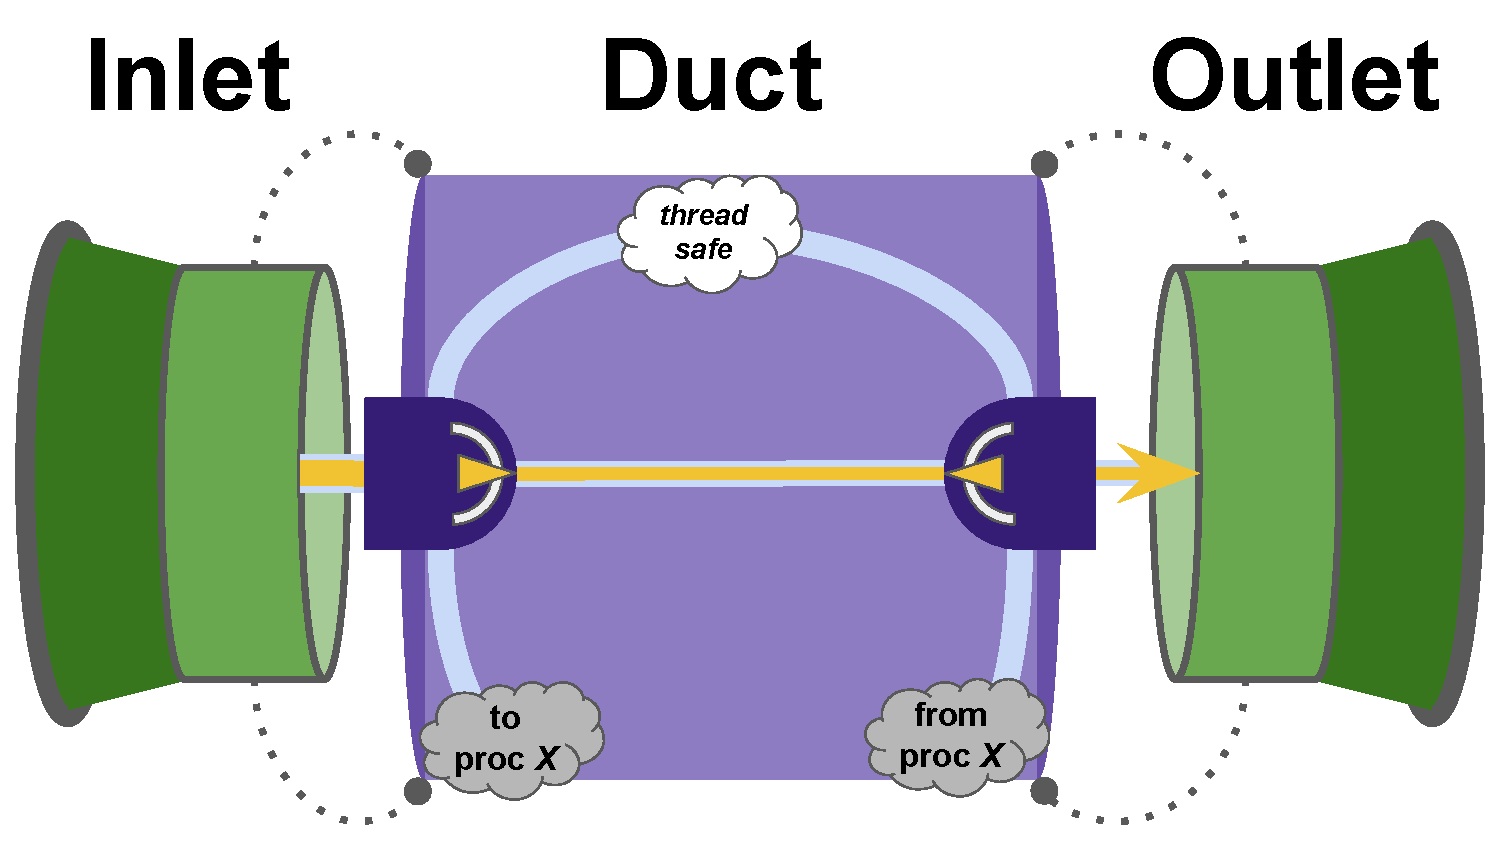
\includegraphics[width=0.8\linewidth]{img/conduit}
      \caption{Schematic of Conduit's \texttt{Inlet} and \texttt{Outlet} object scheme.
      Intra-thread, inter-thread, or inter-process communication behavior is performed by an underlying \texttt{Duct} object.
      The underlying communication mechanism used is transparent to the end-user.
      }
      \label{fig:conduit}
   \end{figure}

The Conduit C++ Library aims to compliment the parallel and distributed programming ecosystem by providing an abstracted best-effort interface to application programmers.
Under Conduit's interface, more recent messages may preempt existing ones, messages may be dropped under backlog conditions, and read operations may opt to view the most recently received message in lieu of waiting for an expected message.

Conduit represents communication in terms of a paired \texttt{Inlet}, which accepts messages, and \texttt{Outlet}, which dispenses messages.
An \texttt{Inlet} and \texttt{Outlet} may exchange messages via an intra-thread, inter-thread, or inter-process communication procedure, depending on the runtime state of an underlying \texttt{Duct} object.
Figure \ref{fig:conduit} provides a schematic overview.
The implementation of intra-thread, inter-thread, and inter-process communication procedures may be configured at compile-time.
Conduit provides a library of intra-thread, inter-thread, and inter-process implementations to choose from and allows end-users to build their own.

The \texttt{Inlet} provides a non-blocking \texttt{TryPut()} method, which attempts to queue a message for its corresponding \texttt{Outlet} but may drop it under backlog conditions, as well as a \texttt{Put()} method, which block under backlog conditions until buffer space is available to queue the message is available.
The \texttt{Outlet} provides a \texttt{TryStep()} and \texttt{Jump()} methods to load the next or latest message, respectively.
If no new messages are available, the last-received message will be accessed.
The \texttt{Outlet} also provides a \texttt{Step()} method, which will block until a new message is received.
At run time, \texttt{Duct}s can be created or modified to perform intrathread, interthread, or interprocess communication. 

In addition to this granular connection-level interface, Conduit provides a network-level interface where the user defines their computation in terms of a directed graph.
In this network topology, nodes represent simulation elements and edges represent communication channels.
The library will assign nodes in that topology to available threads across available processes and automatically instantiate appropriate conduits.
Individual threads of execution can then launch and freely process computational updates on their assigned nodes while receiving messages from nodes assigned to other processes as they become available.
Conduit provides several pre-defined standard topologies and node-assignment algorithms.
However, users can also opt to use the NetworkX graph library \cite{hagberg2008exploring} to generate arbitrary topologies and the METIS software package \cite{gupta1997fast} to automatically balance expected load across available threads and processes while minimizing inter-process and inter-thread communication.

Defining program logic in terms of atomic, inter-communicating simulation elements provides significant programmability advantages.
Such code can be written in terms of interactions between intuitive domain-specific objects (e.g., digital organisms that interact with one another, subpopulations with migration, etc.), while leaving the task of mapping onto hardware resources to automatic management by the underlying framework.
However, a naive implementation of this approach would entail significant inefficiency, particularly with inter-process communication which has a large overhead.
Imagine, for example, a processes dispatching independent MPI calls for each communication channel between another process and the thousands of atomic simulation elements it holds.
Conduit addresses this issue by providing duct implementations that automatically consolidate messages between processes into single MPI calls.
These implementations support a ``pooling'' mechanism, in which a consolidated MPI call is dispatched once each constituent \texttt{Inlet} has received a single message, and a ``aggregation'' mechanism, in which arbitrary numbers of messages can be contributed from each \texttt{Inlet}.

Conduit is made freely available under a MIT License as a header-only C++17 software package at \url{https://github.com/mmore500/conduit}.
Conduit was built using the cereal C++11 Library for serialization \cite{voorhies2017cereal} and the Empirical C++ Library \cite{charles_ofria_2019_2575607}.
